% Digital Logic Report Template
% Created: 2020-01-10, John Miller

%==========================================================
%=========== Document Setup  ==============================

% Formatting defined by class file
\documentclass[11pt]{article}

% ---- Document formatting ----
\usepackage[margin=1in]{geometry}	% Narrower margins
\usepackage{booktabs}				% Nice formatting of tables
\usepackage{graphicx}				% Ability to include graphics

%\setlength\parindent{0pt}	% Do not indent first line of paragraphs 
\usepackage[parfill]{parskip}		% Line space b/w paragraphs
%	parfill option prevents last line of pgrph from being fully justified

% Parskip package adds too much space around titles, fix with this
\RequirePackage{titlesec}
\titlespacing\section{0pt}{8pt plus 4pt minus 2pt}{3pt plus 2pt minus 2pt}
\titlespacing\subsection{0pt}{4pt plus 4pt minus 2pt}{-2pt plus 2pt minus 2pt}
\titlespacing\subsubsection{0pt}{2pt plus 4pt minus 2pt}{-6pt plus 2pt minus 2pt}

% ---- Hyperlinks ----
\usepackage[colorlinks=true,urlcolor=blue]{hyperref}	% For URL's. Automatically links internal references.

% ---- Code listings ----
\usepackage{listings} 					% Nice code layout and inclusion
\usepackage[usenames,dvipsnames]{xcolor}	% Colors (needs to be defined before using colors)

% Define custom colors for listings
\definecolor{listinggray}{gray}{0.98}		% Listings background color
\definecolor{rulegray}{gray}{0.7}			% Listings rule/frame color

% Style for Verilog
\lstdefinestyle{Verilog}{
	language=Verilog,					% Verilog
	backgroundcolor=\color{listinggray},	% light gray background
	rulecolor=\color{blue}, 			% blue frame lines
	frame=tb,							% lines above & below
	linewidth=\columnwidth, 			% set line width
	basicstyle=\small\ttfamily,	% basic font style that is used for the code	
	breaklines=true, 					% allow breaking across columns/pages
	tabsize=3,							% set tab size
	commentstyle=\color{gray},	% comments in italic 
	stringstyle=\upshape,				% strings are printed in normal font
	showspaces=false,					% don't underscore spaces
}

% How to use: \Verilog[listing_options]{file}
\newcommand{\Verilog}[2][]{%
	\lstinputlisting[style=Verilog,#1]{#2}
}




%======================================================
%=========== Body  ====================================
\begin{document}

\title{ELC 2137 Lab 9: ALU}
\author{Jake Simmons}

\maketitle


\section*{Summary}

Type the summary of your experiment and results here.  


\section*{Q\&A}

Answer questions posed in the lab assignment here.


\section*{Results}

\begin{figure}[ht]\centering
	\begin{tabular}{l|rrrrrrrrrrr}
		Time (ns): & 0-5 & 5-10 & 10-15 & 15-20 & 20-25 & 25-30 & 30-35 & 35-40 & 40-45 & 45-50 & 50-55 \\
		\midrule
		D (hex) & 0 & 0 & A & A & 3 & 3 & 0 & 0 & 0$\rightarrow$6 & 6 & 6 \\
		clk & 0 & 1 & 0 & 1 & 0 & 1 & 0 & 1 & 0 & 1 & 0  \\
		en & 0 & 0 & 1 & 1 & 1$\rightarrow$0 & 0$\rightarrow$1 & 1$\rightarrow$0 & 0 & 0$\rightarrow$1 & 1 & 1 \\
		rst & 0 & 0$\rightarrow$1 & 0 & 0 & 0 & 0 & 0 & 0 & 0 & 0 & 0 \\
		\midrule 
		Q (hex) & X & X$\rightarrow$0 & 0 & 0 & 0 & 3 & 0 & 0 & 6 & 0 & 0 \\
		\bottomrule
	\end{tabular}\medskip
	
%	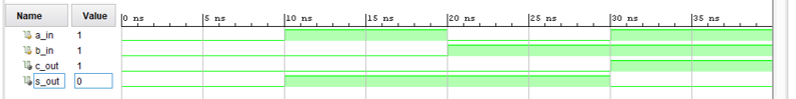
\includegraphics{sim_waveform}
	\caption{ERT and Simultion Waveforms of Register}
%	\label{fig:sim_with_table}
\end{figure}

\begin{figure}[ht]\centering
	\begin{tabular}{l|rrrrrr}
		Time (ns): & 0-10 & 10-20 & 20-30 & 30-40 & 40-50 & 50-60  \\
		\midrule
		in0 (dec) & 5 & 10 & 1 & 3 & 5 & 15 \\
		in1 (dec) & 5 & 5 & 2 & 4 & 6 & 12 \\
		op (dec) & 0 & 1 & 2 & 3 & 4 & 5 \\
		\midrule 
		out (dec) & a & 5 & 0 & 7 & 3 & 15 \\
		\bottomrule
	\end{tabular}\medskip
	
	%	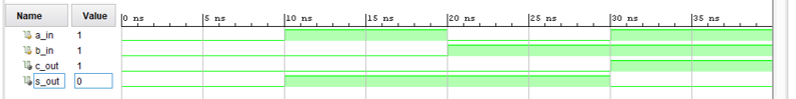
\includegraphics{sim_waveform}
		\caption{ERT and Simulation Waveforms of ALU}
	%	\label{fig:sim_with_table}
\end{figure}



\section*{Code}

Include all of the code you wrote or modified here.


\end{document}
